\chapter{Der Algorithmus}
Es existieren verschiedenste Lernalgorithmen um Elman Netze und im Allgemeinen rekurrente Netze zu trainieren. Vieles h�ngt von der Architektur und der Aufgabenstellung des Netzes ab. Beispiele sind etwa 
\begin{itemize}
	\item der dynamische Backpropagation Algorithmus,
	\item der Real-Time Recurrent Learning Algorithmus
	\item oder die Kalman Filter.
\end{itemize}
In dieser Arbeit wird speziell auf den dynamischen Backpropagation Algorithmus\cite{pham} eingegangen.

\section{Dynamische Backpropagation}
\begin{figure}[H]
	\centering
	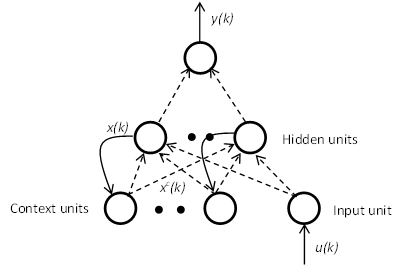
\includegraphics[height=6cm]{BasicElman.png}
	\caption{Basic Elman Network}
	\label{basicElman}
\end{figure}
Abbildung \ref{basicElman} zeigt die Architektur eines klassischen Elman Netzes nach Elman 1990\cite{elman}. Die feedforward-Verbindungen (gestrichelte Linien) sind ver�nderbar und die rekurrenten Verbindungen (geschlossene Linien) sind fix.

\subsection{Berechnung der Neuronen}
Sei der Input des Netzes $u(k)$, der Output $y(k)$, der gesamte Input zu den einem $i$-ten verdeckten Neuron $v_i(k)$, der Output eines $i$-ten verdeckten Neuron $x_i(k)$ und der Output eines $j$-ten Kontextneurons $x_j^c(k)$, dann gilt:
\begin{align}
	v_i(k) &= \sum\limits_{j=1}^n w_{i,j}^x(k-1) x_j^c(k) + w_i^u(k-1) u(k), \tag{1a}\\
	x_i(k) &= f(v_i), \tag{1b}\\
	x_j^c(k) &= x_j(k-1), \tag{1c}\\
	y(k) &= \sum\limits_{i=1}^n w_i^y(k-1) x_i(k), \tag{1d}
\end{align}
wobei $w_i^u, w_{i,j}^x$ und $w_i^y$, $i,j=1,\ldots,n$, die Gewichte der Verbindungen zwischen Input- und verdeckter Schicht, Kontext- und verdeckter Schicht und zwischen verdeckter und Outputschicht sind und $f$ eine sigmoidale Aktivierungsfunktion ist.

Wird nun der Input $u(k)$ um einen Zeitschritt verz�gert, bevor er gesendet wird, wird $x_j^c(k)$ mit $x_j(k-1)$ ersetzt und angenommen die verdeckten Neuronen sind linear, dann gelten folgende Gleichungen:
\begin{align}
	v_i(k) &= \sum\limits_{j=1}^n w_{i,j}^x(k-1) x_j(k-1) + w_i^u(k-1) u(k-1), \tag{2a}\\
	x_i(k) &= v_i(k), \tag{2b}\\
	y(k) &= \sum\limits_{i=1}^n w_i^y(k-1) x_i(k). \tag{2c}
\end{align}
Diese Gleichungen beschreiben ein State-Space Model $n$-ter Ordnung eines linearen dynamischen Systems und k�nnen als folgende Gleichung dargestellt werden:
\begin{align}
	y(k) &= A_1 y(k-1) + A_2 y(k-2) + \cdots + A_n y(k-n) \notag \\
	&+ B_1 u(k-1) + B_2 u(k-2) + \cdots + B_n u(k-n). \tag{3}
\end{align}

\subsection{Training durch dynamische Backpropagation}
Seien die Trainingswerte das Paar $(u(k),y_d(k))$, $k=1,2,\ldots,N$, mit $u(k)$ als Input und $y_d(k)$ als gew�nschter Output.\\
Die Fehlerfunktion des Netzes zum Zeitpunkt $k$ ist
\begin{align}
	E_k = \frac{1}{2} \left(y_d(k)-y(k)\right)^2. \tag{4}
\end{align}
Die Gewichte des Netzes werden zu jedem Zeitpunkt $k$ modifiziert. Der Fehlergradient f�r $w_i^y(k-1)$ ist
\begin{align}
	\frac{\partial E_k}{\partial w_i^y(k-1)} &= -(y_d(k)-y(k)) \frac{\partial y(k)}{\partial w_i^y(k-1)} \notag \\
	&= -(y_d(k)-y(k)) x_i(k). \tag{5}
\end{align}
Die Fehlergradienten f�r $w_i^u(k-1)$ und $w_{i,j}^x(k-1)$ lauten
\begin{align}
	\frac{\partial E_k}{\partial w_i^u(k-1)} &= -\frac{\partial E_k}{\partial y(k)} \frac{\partial y(k)}{\partial x_i(k)} \frac{\partial x_i(k)}{\partial v_i(k)} \frac{\partial v_i(k)}{\partial w_i^u(k-1)} \notag \\
	&= -(y_d(k)-y(k)) w_i^y(k-1) f'(u(k)) \tag{6}
\end{align}
und
\begin{align}
	\frac{\partial E_k}{\partial w_{i,j}^x(k-1)} &= -\frac{\partial E_k}{\partial y(k)} \frac{\partial y(k)}{\partial x_i(k)} \frac{\partial x_i(k)}{\partial w_{i,j}^x(k-1)} \notag \\
	&= -(y_d(k)-y(k)) w_i^y(k-1) \frac{\partial x_i(k)}{\partial w_{i,j}^x(k-1)}, \tag{7}
\end{align}
wobei
\begin{align}
	\frac{\partial x_i(k)}{\partial w_{i,j}^x(k-1)} &= \frac{\partial x_i(k)}{\partial v_i(k)} \frac{\partial v_i(k)}{\partial w_{i,j}^x(k-1)} \notag \\
	&= f'\left(\frac{\partial v_i(k)}{\partial w_{i,j}^x(k-1)}\right) \notag \\
	&= f'\left(x_j(k-1) + \sum\limits_{l=1}^n w_{i,l}^x(k-1) \frac{\partial x_l(k-1)}{\partial w_{i,j}^x(k-2)}\right). \tag{8}
\end{align}

\subsection{Zusammenfassung}
Der dynamische Backpropagation-Algorithmus kann nun wie folgt zusammengefasst werden.\\
\subsubsection{Berechnung der Neuronen:}
\begin{align}
	v_i(k) &= \sum\limits_{j=1}^n w_{i,j}^x(k-1) x_j(k-1) + w_i^u(k-1) u(k), \tag{9a} \\
	x_i(k) &= f(v_i), \tag{9b} \\
	y(k) &= \sum\limits_{i=1}^n w_i^y(k-1) x_i(k). \tag{9c}
\end{align}
\subsubsection{Update der Gewichte:}
\begin{align}
	w_i^y(k) &= w_i^y(k-1) - \eta (y_d(k)-y(k)) x_i(k), \tag{10a} \\
	w_i^u(k) &= w_i^u(k-1) - \eta (y_d(k)-y(k)) w_i^y(k-1) f'(u(k)), \tag{10b} \\
	w_{i,j}^x(k) &= w_{i,j}^x(k-1) - \eta (y_d(k)-y(k)) w_i^y(k-1) \frac{\partial x_i(k)}{\partial w_{i,j}^x(k-1)}, \tag{10c} \\
	\frac{\partial x_i(k)}{\partial w_{i,j}^x(k-1)} &= f'\left(x_j(k-1) + \sum\limits_{l=1}^n w_{i,l}^x(k-1) \frac{\partial x_l(k-1)}{\partial w_{i,j}^x(k-2)}\right). \tag{10d}
\end{align}
